\documentclass[oneside,final,14pt,a4paper]{extreport}

\usepackage{vmargin}
\setpapersize{A4}
\setmarginsrb{2.5cm}{2cm}{2cm}{2cm}{0pt}{10mm}{0pt}{13mm}
\usepackage{setspace}
\sloppy
\setstretch{1.5}
\usepackage{indentfirst}
\parindent=1.25cm

%%%%% ADDED TO SUPPORT TT BOLD FACES %%%%
\DeclareFontShape{OT1}{cmtt}{bx}{n}{<5><6><7><8><9><10><10.95><12><14.4><17.28><20.74><24.88>cmttb10}{}
\renewcommand{\ttdefault}{pcr}
%%%%% END %%%%%%%%%%%%%%%%%%%%%%%%%%%%%%% 
\usepackage{atbegshi,picture}
\usepackage[T1,T2A]{fontenc} 
\usepackage[utf8]{inputenc}
\usepackage[main=russian,english]{babel}
\usepackage[backend=biber,style=ieee,autocite=inline]{biblatex}
\bibliography{ref.bib}
\usepackage{csquotes}
\usepackage{blindtext}
\usepackage{fontspec}
\usepackage{stmaryrd}
\setmainfont{Times New Roman}

\newcommand{\mkObject}[1]{\llbracket #1 \rrbracket}


\usepackage{pdfpages}
\newenvironment{bottompar}{\par\vspace*{\fill}}{\clearpage}

% \usepackage{cite}
\usepackage{amsmath,amsfonts}

\usepackage{amsthm}
\newtheorem{theorem}{Theorem}
\newtheorem{corollary}{Corollary}
\newtheorem{lemma}{Lemma}
\newtheorem{proposition}{Proposition}
\theoremstyle{definition}
\newtheorem{definition}{Definition}
\theoremstyle{remark}
\newtheorem*{remark}{Remark}
\theoremstyle{remark}
\newtheorem*{example}{Example}



\usepackage{graphicx}
\graphicspath{{figs/}} %path to images
\usepackage{array}
\usepackage{multirow,array}
\usepackage{caption}
\usepackage{subcaption}
\usepackage[unicode]{hyperref}
\usepackage{paralist}
\usepackage{listings}
\usepackage{zed-csp}
\usepackage{fancyhdr}
\usepackage{color,colortbl}
\usepackage{booktabs}
\usepackage{epsfig} % for postscript graphics files

\usepackage{upgreek} 
\usepackage{bm}
\usepackage{hyperref}
\usepackage{setspace}
\usepackage{booktabs}
\usepackage{multirow}
\usepackage{longtable}
\usepackage[font=singlespacing, labelfont=bf]{caption}
\usepackage{epsfig} % for postscript graphics files
\counterwithout{table}{chapter}
\renewcommand{\thetable}{\Roman{table}}
\usepackage{floatrow}

\pagestyle{fancyplain}

% remember section title
\renewcommand{\chaptermark}[1]%
	{\markboth{\chaptername~\thechapter~--~#1}{}}

% subsection number and title
\renewcommand{\sectionmark}[1]%
	{\markright{\thesection\ #1}}

\rhead[\fancyplain{}{\bf\leftmark}]%
      {\fancyplain{}{\bf\thepage}}
\lhead[\fancyplain{}{\bf\thepage}]%
      {\fancyplain{}{\bf\rightmark}}
\cfoot{} %bfseries

\newcommand\pic[1]{(Рис. \ref{#1})} %Ref on figure
\newcommand\tab[1]{(Tab. \ref{#1})} %Ref on table
\lstset{escapeinside={(*@}{@*)}}
\definecolor{light-gray}{gray}{0.80}

\newcommand{\dedication}[1]
   {\thispagestyle{empty}
     
   \begin{flushleft}\raggedleft #1\end{flushleft}
}


\begin{document}

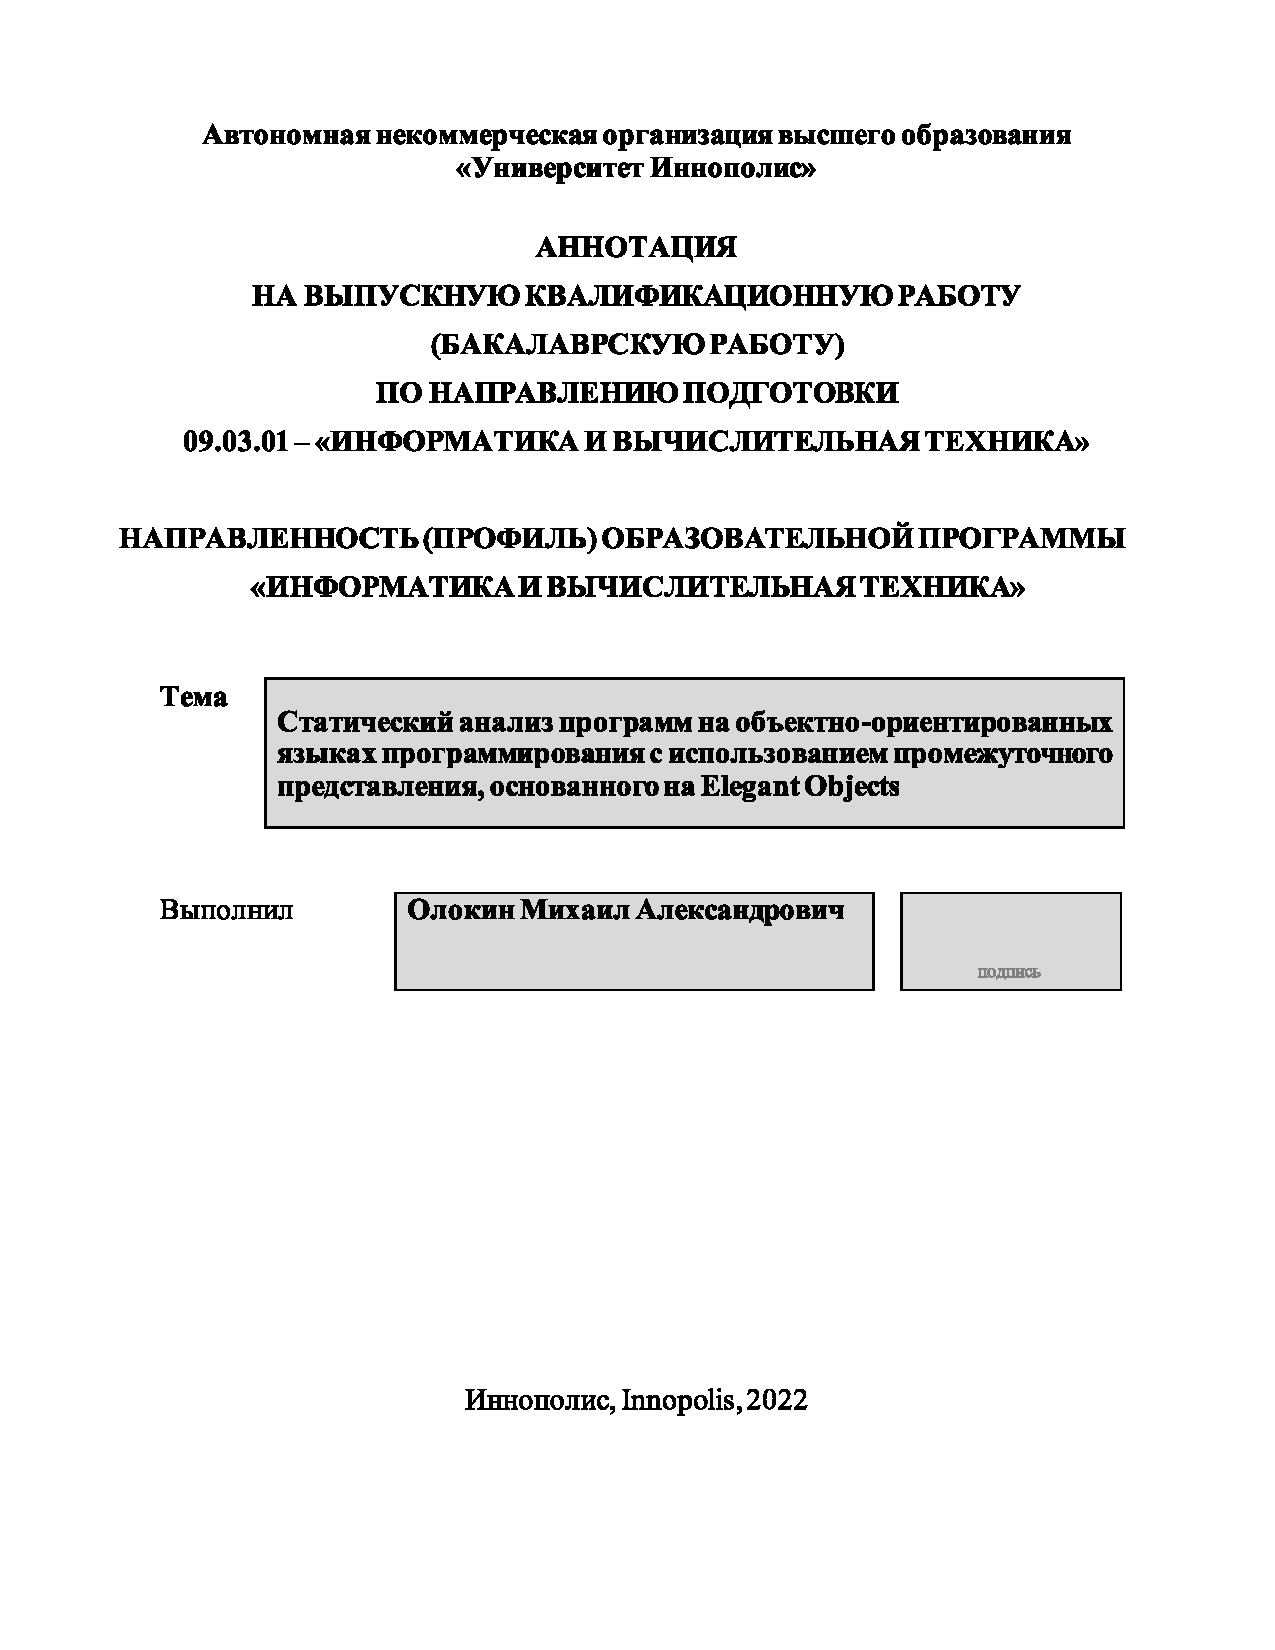
\includepdf[pages=-, offset={-\hoffset} {\voffset}]{annotation_title.pdf}
\AtBeginShipout{\AtBeginShipoutUpperLeft{%
  \put(\dimexpr\paperwidth-1cm\relax,-1.5cm){\makebox[0pt][r]{
\includegraphics[width=3cm]{figs/inno}}}%
}}

\tableofcontents
\newpage
\begin{abstract}

\end{abstract}

\setcounter{page}{5}

\chapter{Introduction}
\label{chap:intro}
\chaptermark{Optional running chapter heading}



\label{sec:section}
Object-oriented programming languages have been adopted widely over the past two decades. As of March 2022, the top five positions of the TIOBE index are occupied by Python, C, Java, C++ and C\#. Four of these languages (with the exception of C) are considered object-oriented and, as the index suggests, are widely adopted and used in large-scale commercial products. 

\section{Properties of Object-Oriented Programming Languages}
According to \cite{oop1}, \textit{object-oriented} programming languages are the languages where the main unit of abstraction is an \textit{object}. Objects encapsulate \textit{data}, which are the values of some type. Some languages, e.g. Java and C++, distinguish between \textit{primitive types}, which represent low-level constructs like numbers or boolean values, and \textit{object types}, which represent a composite type. Objects may also contain operations on the said data, known as \textit{methods}. Methods can take parameters and may return a value. 

Objects should also obey certain definitive properties. As \cite{oop1} suggests, " the extent to which a particular language satisfies these properties defines how much of an object-oriented language it is." These properties are:
\begin{itemize}
    \item Encapsulation - an object should expose a well-defined interface through which it should be consumed. The irrelevant details of how an object implements this interface should be \textit{hidden} from the consumer.
    \item Inheritance - is a mechanism through which objects can share functionality and extend the behavior of other objects. Inheritance is a complex mechanism and its implementation differs from language to language. As per \cite{oop1}, "Inheritance enables programmers to reuse the definitions of previously defined structures. This clearly reduces the amount of work required in producing".
    \item Polymorphism - a possibility to define operations on objects in such a way, that they can accept and return values of multiple types. 
    \item Dynamic (or late \cite{alankay}) binding - the implementation of the method to be run on an object is chosen at runtime. This implies that the implementation that is used during the runtime of a program may be \textit{different} from that of a type that is known statically (i.e. at compile time)

\end{itemize}

\section{Criticism}

Together with increasing adoption, OO programming techniques and languages have gained a substantial amount of valid criticism. Mansfield \cite{oopfailed} mentions most of these complaints, ultimately claiming that "...with OOP-inflected programming languages, computer software becomes more
verbose, less readable, less descriptive, and harder to modify and maintain". Many of these criticisms are being turned into recommendations, such as the famous "Design patterns: elements of reusable object-oriented software" \cite{GOFPatterns}. However, such recommendations are not the part of the language specification and thus can not be enforced by the language compiler. This leads to these recommendations often being misinterpreted or overused, especially by beginning software engineers.

\section{Analysis Tools}
To mitigate this complexity and enforce good practices, developers have created a lot of software tools. These tools can be divided into two categories: \textit{dynamic analyzers} and \textit{static analyzers}. 

\textit{Dynamic analyzers} (also known as \textit{profilers}) inspect the state of the program as it is being executed. Dynamic analyzers collect important information about the program execution, such as CPU utilization and memory consumption and present it in the human-readable form. This information is crucial in applications where the performance plays an important role. Unfortunately, the tools require the program under analysis to be executed, which can be expensive or even impossible, e.g. when the program is to be run on dedicated hardware. 

On the contrary, \textit{static analyzers} inspect the source code of the program (or one of its intermediate representations) \textit{without executing it} to locate common errors, anti-patterns and deviations from the accepted style conventions. Executing such tools isn't usually time-consuming or otherwise expensive, which is why they are a crucial part of continuous integration (CI) pipelines and integrated development environments (IDEs). 
Despite being prone to false positives, static analysis tools can pinpoint the location of the error with greater precision.

Unlike dynamic analyzers, static analyzers operate on the source code, which allows them to inspect the program from a higher-level perspective. This means that static analyzers can improve the error reporting of programming language compilers, discover more problems, and  even automatically fix them.

Prior to analysis, many static analysis tools convert the source of the target language into some intermediate representation. This is done for several reasons. In general, this is done to extract the information from the source code that is relevant for analysis needs. Another common use case for employing an intermediate representation would be to
make the static analyzer work with more than one target language. In this case the representation serves as a common ground for the various analyzers. The examples of  intermediate representation are LLVM \cite{llvm} and Jimple \cite{vallee1998jimple} (used in SOOT \cite{vallee2010soot}).

\section{Research Objective}

In this thesis we present an implementation of a static analyzer for object-oriented programming languages with Elegant Objects \cite{eolang} (or EO) as an intermediate representation. This representation is based on $\phi$-calculus, a formal model that is designed to unify the varying semantics of object-oriented (OO) languages. It also claims to be a language with minimum verbosity, providing only the required subset of operators. The combination of a strict formal ground and a reduced feature set make EO a powerful intermediate representation for a static analyzer that should be able to capture many bugs specific to OO programs. 

The rest of this thesis is structured as follows: Chapter 2 covers the existing work of finding bugs in OO programs, the semantics of EO and how it represents OO programs, Chapter 3 describes the implementation of the analyzer, Chapter 4 covers the evaluation of the analyzer, including testing and benchmarks and, finally, Chapter 5 concludes the thesis.

\chapter{Literature Review}
\label{chap:lr}
\chaptermark{Second Chapter Heading}
Static analysis of object-oriented programs is a well-studied area. However, most of the effort in these studies was focused on analysing specific languages.

One of these areas is the . This area is crucial for this thesis, because it motivates the existence of the tool we are trying to create. Another area of interest may be "attempts to establish a formal foundation for object-oriented languages". This is the area where we may find how EO intersects with other similar works in the area and what sets it apart. 
\section{Navigation}

\section{Methods \& Criteria}

\section{Fragile Base Class Problem}

\section{Intermediate Representations for Static Analyzers}

\section{Formalizations of Object-oriented Programming}



\newpage

\chapter{Methodology}
\label{chap:met}


Referencing other chapters \ref{chap:lr}, \ref{chap:met}, \ref{chap:impl}, \ref{chap:eval} and \ref{chap:conclusion}

\section{Describing object-oriented programs with EOLANG}

\section{}
\chapter{Implementation}
\label{chap:impl}
This chapter analyzes specifics of Odin (short for Object Dependency INspector) - a static analyzer of EO source code. Section 4.1 covers the tools and technologies used in the project. Section 4.2 gives a brief overview of the project file structure.
Section 4.3 goes over the implementation of EO parser used in the project. Section 4.4 discusses the ways we can represent the elements of object-oriented programs in EO. Sections 4.5 and 4.6 describe the implementations of the analysis algorithms applied to structured EO code. Finally, section 4.7 summarizes this chapter.

\section{Development Environment}
Odin is a project written entirely in Scala [15] - a modern programming language with support for high-level concepts such as structural pattern matching and algebraic data types. Scala is compiled into Java Virtual Machine (JVM) byte code. This allows Odin to be used as a library in any other project compatible with JVM, be it Scala or Java. In addition, programs compiled to JVM byte code can be run without changes on any device that can run Java Virtual Machine.


The project uses a build tool called sbt. sbt allows compiling multiple Scala modules at once. A distinctive feature of sbt is the ability to compile Scala code in a way that makes it compatible with many Scala versions [16]. It also supports a variety of plugins that improve the development process. The plugins used by Odin are scalafmt, an automatic code formatter for scala, and scalafix, a linter and code analyzer with support for project-wide refactorings.

Odin is published as a JAR [17] and distributed through Maven Central [18].

The source code of the project is available on Github [19].



\section{Module Structure}
Odin is a project consisting of multiple modules. The main modules are:
\begin{itemize}
    \item Core, which contains the definition for EO AST (Abstract Syntax Tree).
          This AST is used as an input to all analysis algorithms.
    \item Analyses, which contains the implementations of various analyzers.
    \item Backends, which contains algorithms that transform EO AST into something else. The only backend so far is a plain text backend: it transforms EO AST into its syntactically correct equivalent in EO source code. This backend can also be interpreted as a pretty-printer of EO code and is widely used as such in other modules.
    \item Parser, which contains a parser (also known as a syntactic analyzer) of EO source code. It is used to convert different EO representations (e.g. plain text or XML encoding) into the EO AST defined in Core module.
\end{itemize}
\section{Parser}
The parser used in Odin implements a slightly altered version of EO specification defined by Bugayenko [23]. In particular, it relaxes constraints on whitespace between tokens and the number of newlines and comments between definitions. This is done to reduce the complexity of producing source code pieces for testing and debugging.

The parser was created using cats-parse library [24] for Scala. It provides a parser-combinator [25] approach to building recursive-descent parsers. Recursive-descent parsers are known for their worst-case exponential complexity. This problem can not be avoided in general. However, cats-parse mitigates it by explicitly marking all the places in the parser definition that can cause such spikes in complexity.

\section{Representing Object-Oriented Programming Concepts in EO}
Before analyzing programs written in object-oriented (OO) programming languages, it is necessary to translate them into EO while preserving the semantics of the original language. This chapter presents a version of such an encoding that is assumed by Odin.

\subsection{Classes}
Classes are modelled as EO objects that do not take any parameters. Class-level (i.e. "static") attributes become attributes of the class object. Constructor is represented by an attribute-object "new" of the class object. This object may take parameters to produce an instance of the object.

All instance attributes and methods are defined inside the object returned by the "new" object. Inheritance is modelled as decoration in EO. So, a full example of EO translation would look like this. Class instances (a.k.a objects in Java) are created
by instantiating the "new" object with the required parameters.


\subsection{Methods}
Methods are modelled as EO objects, similarly to classes. These objects can take parameters. Instance methods are required to accept a special "self" attribute in addition to other parameters. This parameter is used to pass an instance of the object calling the method (hence the name - "self"). "self" parameter can be used to call instance methods inside other instance methods.

The return value of the method is represented by the value of the $\Phi$ attribute ("@" symbol in EO). In order to call the instance method we need to instantiate the object first. Then we can call the method by accessing the instance's attribute with the method name and passing the instance object to it as the first argument.


\section{Analyses}
This section describes each of the analysis algorithms in greater detail. First, we will describe the steps that are performed prior to each of the defect-specific analyses: parsing and detecting the significant features of EO programs - objects, methods and extension clauses. Then we will describe the algorithms for detecting each of the covered defects: unanticipated mutual recursion and unjustified assumption in subclass. Finally, we will conclude the chapter by describing the shortcomings of each of the algorithms.


\subsection{Preprocessing}
Before running on


\subsection{Unanticipated Mutual Recursion}
Mutual recursion analysis deals with the following problem: suppose we have an object named Base with two methods - $f$ and $g$. Method $g$ calls method $f$, whereas $f$ does something else.


Then, there is a class called Derived that extends Base and redefines the method $f$ in a way that it calls $g$. When we call a method $f$ on an instance of Derived, we get a stack overflow error: method $f$ calls method $g$, method $g$ calls method $f$ and so on (figure \ref{fig:mutualrec_basic}).


\begin{figure}
    \centering
    \begin{subfigure}{0.4\textwidth}
        \lstinputlisting[language=Java]{code/mutualrec.java}
        \caption{Java}
    \end{subfigure}
    \hfill
    \begin{subfigure}{0.4\textwidth}
        \lstinputlisting{code/mutualrec.eo}
        \caption{EO}
    \end{subfigure}
    \caption{Example of unanticipated mutual recursion}
    \label{fig:mutualrec_basic}
\end{figure}

\subsection{Unjustified Assumption Analysis}

\subsection{Shortcomings of the algorithms}

\chapter{Evaluation and Discussion}
\label{chap:eval}
\section{Testing}

\section{Benchmarks}


\ldots



\printbibliography[heading=bibintoc,title={Список литературы}]
\end{document}

